\documentclass[11pt]{article}

\usepackage[margin=1in]{geometry}
\usepackage{amsmath,amssymb}
\usepackage{booktabs}
\usepackage{array}
\usepackage{longtable}
\usepackage{graphicx}
\usepackage{hyperref}

\newcommand{\hashsplit}[2]{{\scriptsize\ttfamily #1}\\{\scriptsize\ttfamily #2}}

\title{Materials Bridge Line A: Ferron Coherence Recoverability Probe for HAOS-IIP}
\author{Tomislav Rupi\'c \\ Independent Researcher}
\date{May 2026}

\begin{document}

\maketitle

\begin{abstract}
This numbered update records release \texttt{64.1}: Materials Bridge Line A for HAOS-IIP. The bridge is an external-data sidecar experiment over published ferron / NbOI$_2$ source data, not a frozen-core modification and not a proof of HAOS-IIP. The runner downloads the Figshare source-data record for Choe et al., ``Observation of coherent ferron emission and propagation,'' parses three public XLSX files, extracts time traces and spectra, and applies bounded HAOS-style recoverability proxies to coherent polarization-wave readouts. The validation status is \texttt{PASS} as an external-data bridge: \texttt{data\_status=REAL\_DATA\_LOADED}, three raw source files are hashed and preserved, nine time traces and six spectra or peak records are parsed, and the recoverability sweep runs deterministically. A second-pass spectral audit finds the target-window feature in \texttt{15/15} audited spectral records near \(3.13\,\mathrm{THz}\), with mean peak frequency \texttt{3.13893 THz}, mean spectral recoverability \texttt{0.928455}, and no detected \(k_\star\) collapse under the current proxy thresholds. A raw STFT/time-frequency audit inspects the XLSX files and returns \texttt{NO\_STFT\_DATA\_FOUND}: one STFT-like sheet is present, but it lacks a usable frequency axis or validated time-frequency grid, so no raw STFT recoverability claim is made. The same Fig. 2d sheet is parsed separately as published post-processed target-band STFT intensity traces: eight traces and 216 time points support a bounded propagation audit with group-velocity proxies of \(58.8\,\mathrm{km/s}\) for \(96\,\mathrm{nm}\) and \(100\,\mathrm{km/s}\) for \(224\,\mathrm{nm}\). A derived, computed-from-time-trace STFT diagnostic over the raw Fig. 2a/2b traces gives mean envelope correlation \texttt{0.995318} against the published target-band traces and mean computed group velocity \texttt{101754 m/s}. A final unified persistence ledger reports \texttt{ferron\_persistence\_proxy=0.957192} while preserving \texttt{raw\_stft\_time\_frequency\_grid\_status=NO\_STFT\_DATA\_FOUND}. The safe claim is that HAOS-IIP now has one external materials-data bridge pipeline that touches real published material-coherence data, records provenance, runs bounded telemetry, and can say both yes and no without overclaiming.
\end{abstract}

\tableofcontents

\section{Status and Scope}

This paper is release \texttt{64.1} in the HAOS-IIP numbered paper sequence.
It records:

\begin{itemize}
\item a new external-data sidecar experiment;
\item public Figshare data ingestion;
\item raw-file preservation and SHA256 manifesting;
\item conservative parsing of source-data XLSX workbooks;
\item bounded recoverability telemetry over ferron / NbOI$_2$ coherent readouts;
\item a second-pass spectral feature audit near \(3.13\,\mathrm{THz}\);
\item a raw STFT/time-frequency audit that records absence of usable STFT grids without fabricating data;
\item a bounded published target-band STFT intensity trace audit over Fig. 2d;
\item a derived computed-from-time-trace STFT diagnostic over raw Fig. 2a/2b traces;
\item a unified ferron harmonic-address persistence summary that preserves the raw-grid boundary;
\item a validation result that preserves the absence of collapse.
\end{itemize}

The sidecar path is:

\begin{quote}
\path{experiments/materials_bridge/ferron_coherence_demo/}
\end{quote}

The bridge does not modify:

\begin{itemize}
\item \path{haos_core};
\item frozen phase folders;
\item frozen telemetry definitions;
\item theory files;
\item existing experiments;
\item prior paper releases.
\end{itemize}

\section{Strict Non-Claims}

This release does not claim:

\begin{itemize}
\item that ferrons prove HAOS-IIP;
\item that ferrons embody HAOS-IIP;
\item a new materials theory;
\item a quantum-consciousness statement;
\item an Orch-OR statement;
\item that recoverability proxies are final physical observables;
\item that a missing \(k_\star\) is a universal coherence guarantee.
\end{itemize}

The narrower question is:

\begin{quote}
Can HAOS-style recoverability metrics be applied to published ferron / NbOI$_2$ coherent polarization-wave data without fabricating data or forcing a positive collapse result?
\end{quote}

\section{Public Data Source}

The primary external source is:

\begin{itemize}
\item Choe et al., ``Observation of coherent ferron emission and propagation,'' \emph{Nature Materials}, 2026, DOI \href{https://doi.org/10.1038/s41563-026-02597-4}{\texttt{10.1038/s41563-026-02597-4}}.
\item Source data DOI: \href{https://doi.org/10.6084/m9.figshare.31895293}{\texttt{10.6084/m9.figshare.31895293}}.
\end{itemize}

The secondary interpretive reference is:

\begin{itemize}
\item Wang et al., ``Ultrafast dynamics of ferroelectric polarization of NbOI$_2$ captured with femtosecond electron diffraction,'' \emph{Nature Communications}, 2025, DOI \href{https://doi.org/10.1038/s41467-025-63533-9}{\texttt{10.1038/s41467-025-63533-9}}.
\end{itemize}

\subsection{Downloaded Raw Files}

The runner downloaded and preserved three raw Figshare XLSX files:

\begin{longtable}{p{0.30\linewidth}p{0.12\linewidth}p{0.46\linewidth}}
\toprule
File & Size & SHA256 \\
\midrule
\endhead
\path{Source data Fig.1.xlsx} & 129205 & \hashsplit{05a38cc576816479f851c0f4dfbe6370}{bed3ca163043e2c386c546980b9e82f3} \\
\path{Source data Fig.2.xlsx} & 420687 & \hashsplit{8cba21ae3cba830a63a71a997532d892}{669139e3ecc7ba73833b53227a81dc25} \\
\path{Source data Fig.4.xlsx} & 5194876 & \hashsplit{42ea381f87d9046fbacce64246324d7b}{33599e5289fb25430bbad2c74f7fa93e} \\
\bottomrule
\end{longtable}

Raw files live under:

\begin{quote}
\path{experiments/materials_bridge/ferron_coherence_demo/outputs/raw/}
\end{quote}

They are not modified by the parser.

\section{HAOS Translation}

The bridge maps the materials readout into HAOS-style telemetry as follows:

\begin{longtable}{p{0.26\linewidth}p{0.62\linewidth}}
\toprule
HAOS-facing term & Materials-side read \\
\midrule
\endhead
carrier & ferroelectric polarization order \\
perturbation & laser pulse, distance, thickness, fluence, temperature, boundary or disorder effects when present \\
recoverable structure & coherent ferron / polarization-wave mode \\
observable readout & narrow-band THz emission, 3.13 THz amplitude, transient reflectance oscillation, Fourier or STFT peak \\
visible failure & loss of narrow-band signal, spectral broadening, amplitude collapse, incoherent background dominance, or propagation failure \\
\bottomrule
\end{longtable}

This is a measurement dictionary, not a materials ontology.

\section{Metric Definitions}

The sidecar computes bounded proxies:

\begin{itemize}
\item \(\texttt{ferron\_peak\_recoverability}\): normalized peak amplitude times peak-frequency stability times linewidth stability;
\item \(\texttt{propagation\_recoverability}\): survival of coherent amplitude across distance when distance metadata exists;
\item \(\texttt{temporal\_recoverability}\): time-trace coherence proxy when delay/time traces are parsed;
\item \(\texttt{combined\_recoverability}\): mean of available recoverability channels;
\item \(\Delta P\): change in combined recoverability between successive conditions;
\item \(k_\star\): first sustained recoverability collapse below threshold \texttt{0.70} for two consecutive steps;
\item \(\texttt{safety\_margin}\): remaining distance from a condition to \(k_\star\), when \(k_\star\) exists;
\item \(\texttt{confidence}\): signal clarity proxy from peak-to-background or strongest persistence drop;
\item \(\texttt{visible\_failure}\): stricter readout failure flag.
\end{itemize}

The important ordering rule is:

\[
k_\star \quad \text{may occur before visible failure.}
\]

That is the bridge test. In this release, \(k_\star\) does not occur.

\section{Validation Result}

\begin{center}
\begin{tabular}{ll}
\toprule
Field & Value \\
\midrule
Validation status & \texttt{PASS} \\
Data status & \texttt{REAL\_DATA\_LOADED} \\
External source data & \texttt{10.6084/m9.figshare.31895293} \\
Files loaded & \texttt{3} \\
Time traces parsed & \texttt{9} \\
Spectra or peak records parsed & \texttt{6} \\
STFT maps parsed & \texttt{0} \\
Baseline recoverability & \texttt{1.0} \\
\(k_\star\) level & \texttt{None} \\
First visible failure level & \texttt{None} \\
Early detection & \texttt{False} \\
Spectral audit status & \texttt{PARTIAL} \\
STFT audit status & \texttt{NO\_STFT\_DATA\_FOUND} \\
Published target-band trace status & \texttt{PASS} \\
Computed STFT diagnostic status & \texttt{PASS} \\
Unified persistence summary status & \texttt{PASS} \\
\bottomrule
\end{tabular}
\end{center}

The confidence summary is:

\begin{center}
\begin{tabular}{ll}
\toprule
Statistic & Value \\
\midrule
Minimum & \texttt{0.8654037886} \\
Mean & \texttt{0.9798696276} \\
Maximum & \texttt{0.9999926836} \\
\bottomrule
\end{tabular}
\end{center}

\section{Distance-Series Read}

The parsed Fig. 2 distance traces provide the closest match to the intended propagation probe. Two distance-series groups are parsed at \(0,2,4,6\,\mu\mathrm{m}\).

\begin{longtable}{p{0.18\linewidth}p{0.12\linewidth}p{0.17\linewidth}p{0.20\linewidth}p{0.18\linewidth}}
\toprule
Series & Distance & Peak frequency & Peak recoverability & Combined recoverability \\
\midrule
\endhead
Fig.2a & \(0\,\mu\mathrm{m}\) & \texttt{3.132363132} & \texttt{1.0000000000} & \texttt{1.0000000000} \\
Fig.2a & \(2\,\mu\mathrm{m}\) & \texttt{3.132363132} & \texttt{1.0000000000} & \texttt{1.0000000000} \\
Fig.2a & \(4\,\mu\mathrm{m}\) & \texttt{3.139293139} & \texttt{0.9778761062} & \texttt{0.9926253687} \\
Fig.2a & \(6\,\mu\mathrm{m}\) & \texttt{3.139293139} & \texttt{0.7519864998} & \texttt{0.9173288333} \\
Fig.2b & \(0\,\mu\mathrm{m}\) & \texttt{3.132363132} & \texttt{1.0000000000} & \texttt{1.0000000000} \\
Fig.2b & \(2\,\mu\mathrm{m}\) & \texttt{3.132363132} & \texttt{1.0000000000} & \texttt{1.0000000000} \\
Fig.2b & \(4\,\mu\mathrm{m}\) & \texttt{3.139293139} & \texttt{0.7519864998} & \texttt{0.9173288333} \\
Fig.2b & \(6\,\mu\mathrm{m}\) & \texttt{3.139293139} & \texttt{0.7519864998} & \texttt{0.9173288333} \\
\bottomrule
\end{longtable}

The current thresholds do not mark a sustained collapse. This is the result: the bridge is operational, the external data is real, and the measured proxy does not force an early-failure story.

\section{Second-Pass Spectral Feature Audit}

The second-pass spectral audit asks a narrower question:

\begin{quote}
What spectral features stand out in the real ferron / NbOI$_2$ data, and do they remain recoverable under the available conditions?
\end{quote}

The audit does not change the first-pass recoverability result. It inspects parsed spectra directly and also records spectra derived from parsed time traces as derived diagnostics, not raw STFT maps.

\begin{center}
\begin{tabular}{ll}
\toprule
Field & Value \\
\midrule
Spectral audit status & \texttt{PARTIAL} \\
Audited spectral records & \texttt{15} \\
Target-window peaks found & \texttt{15/15} \\
Target frequency & \texttt{3.13 THz} \\
Search window & \(\pm\,\texttt{0.20 THz}\) \\
Mean peak frequency & \texttt{3.13893 THz} \\
Peak-frequency range & \texttt{3.13236--3.192 THz} \\
Mean spectral recoverability & \texttt{0.928455} \\
Linewidth proxy availability & \texttt{14/15 records} \\
Mean linewidth proxy & \texttt{0.0253178 THz} \\
Peak-to-background availability & \texttt{14/15 records} \\
Mean peak-to-background & \texttt{8194.98} \\
Spectral \(k_\star\) detected & \texttt{False} \\
Visible failure detected & \texttt{False} \\
\bottomrule
\end{tabular}
\end{center}

The \texttt{PARTIAL} status is intentional. It means the spectral peak audit succeeds, but one record does not support the linewidth or peak-to-background proxy. The audit does not fill those missing quantities.

The bounded read is:

\begin{quote}
A stable target-window peak near \(3.13\,\mathrm{THz}\) appears across the audited records. Peak frequency remains stable under the available conditions. No sustained \(k_\star\) collapse is detected under the current proxy thresholds.
\end{quote}

\section{Raw STFT / Time-Frequency Audit}

The STFT audit asks whether the downloaded XLSX files contain a usable raw time-frequency map. The rule is strict: time traces may not be converted into synthetic STFT maps and then reported as raw STFT data.

\begin{center}
\begin{tabular}{ll}
\toprule
Field & Value \\
\midrule
STFT audit status & \texttt{NO\_STFT\_DATA\_FOUND} \\
Raw XLSX files inspected & \texttt{3} \\
Candidate STFT-like sheets inspected & \texttt{1} \\
Accepted raw STFT maps & \texttt{0} \\
STFT time points audited & \texttt{0} \\
STFT target peak records found & \texttt{0} \\
Mean STFT recoverability & \texttt{None} \\
STFT \(k_\star\) detected & \texttt{False} \\
\bottomrule
\end{tabular}
\end{center}

The one STFT-like candidate is:

\begin{quote}
\path{Source data Fig.2.xlsx#Fig.2d}
\end{quote}

It is rejected because it contains time plus \texttt{STFT Int} columns but no usable frequency axis and no validated time-frequency amplitude grid:

\begin{quote}
\texttt{long\_form\_frequency\_column\_missing; matrix\_axes\_not\_numeric\_enough}
\end{quote}

Therefore, this release makes no STFT recoverability claim. The absence of a parsed raw STFT grid is not treated as negative evidence against the material system; it is only a data-format boundary for this sidecar.

\section{Published STFT Target-Band Intensity Trace Audit}

The rejected raw-STFT candidate is still scientifically useful in a narrower
form. The sheet \path{Source data Fig.2.xlsx#Fig.2d} exports published,
post-processed \texttt{STFT Int} traces in the target band. These traces are
not raw time-frequency maps because no frequency axis is present, so the sidecar
parses them separately as:

\begin{quote}
\texttt{published\_stft\_target\_band\_intensity\_trace}
\end{quote}

This preserves the raw-grid boundary while allowing a bounded propagation-readout
audit over the published target-band envelope.

\begin{center}
\begin{tabular}{ll}
\toprule
Field & Value \\
\midrule
Published trace audit status & \texttt{PASS} \\
Mode & \texttt{published\_stft\_target\_band\_intensity\_trace} \\
Source sheet & \texttt{Source data Fig.2.xlsx\#Fig.2d} \\
Traces found & \texttt{8} \\
Time points audited & \texttt{216} \\
Peak records & \texttt{8} \\
Thickness groups & \texttt{2} \\
Mean group velocity & \texttt{79411.8 m/s} \\
Mean velocity consistency with \(10^5\,\mathrm{m/s}\) & \texttt{0.794118} \\
Mean envelope recoverability & \texttt{0.625} \\
Raw STFT grid status & \texttt{NO\_STFT\_DATA\_FOUND} \\
\bottomrule
\end{tabular}
\end{center}

\begin{longtable}{p{0.16\linewidth}p{0.18\linewidth}p{0.18\linewidth}p{0.16\linewidth}p{0.16\linewidth}}
\toprule
Thickness & Slope & Group velocity & \(R^2\) & Monotonic delay \\
\midrule
\endhead
\(96\,\mathrm{nm}\) & \texttt{17 ps/um} & \texttt{58823.5 m/s} & \texttt{0.955372} & \texttt{1.0} \\
\(224\,\mathrm{nm}\) & \texttt{10 ps/um} & \texttt{100000 m/s} & \texttt{0.987654} & \texttt{1.0} \\
\bottomrule
\end{longtable}

The bounded read is that peak arrival time increases with distance in the
parsed thickness groups. This supports a propagation-readout audit of the
published target-band envelope only. It does not convert the sheet into a raw
STFT grid and it does not create an STFT recoverability claim over a missing
time-frequency amplitude map.

\section{Computed From Time-Trace STFT Diagnostic}

The sidecar also computes a derived diagnostic from the raw Fig. 2a and Fig. 2b
transient-reflectance traces. This diagnostic applies a \(10\,\mathrm{ps}\)
window and \(5\,\mathrm{ps}\) step, extracts intensity near
\(3.13\,\mathrm{THz}\) with a \(\pm 0.05\,\mathrm{THz}\) target band, and compares
the derived envelopes to the published Fig. 2d target-band traces.

This diagnostic is explicitly labeled:

\begin{quote}
\texttt{computed\_from\_time\_trace\_stft\_diagnostic}
\end{quote}

It is not raw published STFT data and it is not used to erase the
\texttt{NO\_STFT\_DATA\_FOUND} boundary.

\begin{center}
\begin{tabular}{ll}
\toprule
Field & Value \\
\midrule
Computed diagnostic status & \texttt{PASS} \\
Source sheets & \texttt{Fig.2a, Fig.2b} \\
Window / step & \texttt{10 ps / 5 ps} \\
Target band & \texttt{3.13 THz +/- 0.05 THz} \\
Traces computed & \texttt{8} \\
Time points computed & \texttt{216} \\
Peak records & \texttt{8} \\
Mean group velocity & \texttt{101754 m/s} \\
Mean envelope correlation vs. published & \texttt{0.995318} \\
Mean absolute peak-time delta vs. published & \texttt{5.84163 ps} \\
Raw STFT grid status & \texttt{NO\_STFT\_DATA\_FOUND} \\
\bottomrule
\end{tabular}
\end{center}

\begin{longtable}{p{0.16\linewidth}p{0.18\linewidth}p{0.18\linewidth}p{0.16\linewidth}p{0.16\linewidth}}
\toprule
Thickness & Slope & Group velocity & \(R^2\) & Monotonic delay \\
\midrule
\endhead
\(224\,\mathrm{nm}\) & \texttt{7.5 ps/um} & \texttt{133333 m/s} & \texttt{1.0} & \texttt{1.0} \\
\(96\,\mathrm{nm}\) & \texttt{14.25 ps/um} & \texttt{70175.4 m/s} & \texttt{0.998157} & \texttt{1.0} \\
\bottomrule
\end{longtable}

The raw Fig. 2a/Fig. 2b headers do not include thickness labels. The sheet
assignment follows the published Fig. 2d propagation peak-time ordering and is
therefore recorded as an assignment rule, not as independent metadata discovery.

\section{Unified Harmonic-Address Persistence Summary}

The final sidecar layer gathers the spectral, published-trace, computed-STFT,
and raw-grid-boundary outputs into one component ledger. This is a summary of
already bounded outputs, not a new materials theory.

\begin{center}
\begin{tabular}{ll}
\toprule
Field & Value \\
\midrule
Persistence summary status & \texttt{PASS} \\
Mode & \texttt{ferron\_harmonic\_address\_persistence\_summary} \\
Target frequency & \texttt{3.13 THz} \\
Combined persistence proxy & \texttt{0.957192} \\
Raw STFT grid status & \texttt{NO\_STFT\_DATA\_FOUND} \\
Raw grid boundary preserved & \texttt{True} \\
\bottomrule
\end{tabular}
\end{center}

\begin{longtable}{p{0.32\linewidth}p{0.15\linewidth}p{0.18\linewidth}p{0.24\linewidth}}
\toprule
Component & Value & Included & Source \\
\midrule
\endhead
\texttt{target\_peak\_presence} & \texttt{1.0} & yes & spectral audit \\
\texttt{spectral\_recoverability} & \texttt{0.928455} & yes & spectral audit \\
\texttt{no\_sustained\_k\_star} & \texttt{1.0} & yes & spectral audit \\
\texttt{published\_propagation\_monotonicity} & \texttt{1.0} & yes & published trace audit \\
\texttt{published\_velocity\_consistency} & \texttt{0.794118} & yes & published trace audit \\
\texttt{computed\_envelope\_match} & \texttt{0.995318} & yes & computed STFT diagnostic \\
\texttt{computed\_velocity\_consistency} & \texttt{0.982456} & yes & computed STFT diagnostic \\
\texttt{raw\_stft\_grid\_boundary} & \texttt{None} & no & raw STFT audit \\
\bottomrule
\end{longtable}

The raw-grid boundary is excluded from the numeric proxy. It is a
data-availability boundary, not a persistence penalty. The bounded
interpretation is:

\begin{quote}
The ferron sidecar shows a stable target-window spectral feature near
\(3.13\,\mathrm{THz}\), published target-band STFT intensity traces with
monotonic propagation delay, and computed-from-time-trace STFT envelopes that
closely match the published traces. The raw STFT time-frequency grid remains
unavailable in the downloaded XLSX files; that boundary is preserved. This is
a bounded external-data persistence summary, not a proof or materials-theory
claim.
\end{quote}

\section{Figures}

\begin{figure}[ht]
\centering
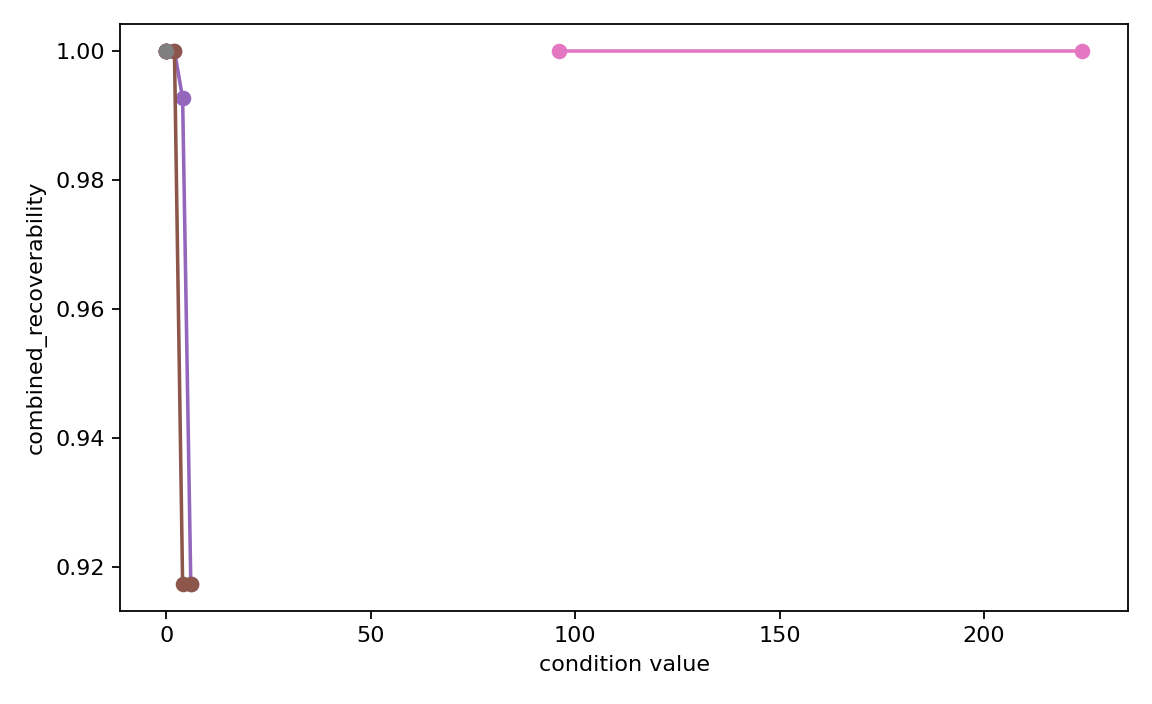
\includegraphics[width=0.88\linewidth]{../experiments/materials_bridge/ferron_coherence_demo/outputs/recoverability_vs_condition.png}
\caption{Combined recoverability versus parsed condition. The distance-series traces remain above the configured collapse threshold under the current proxy setup.}
\end{figure}

\begin{figure}[ht]
\centering
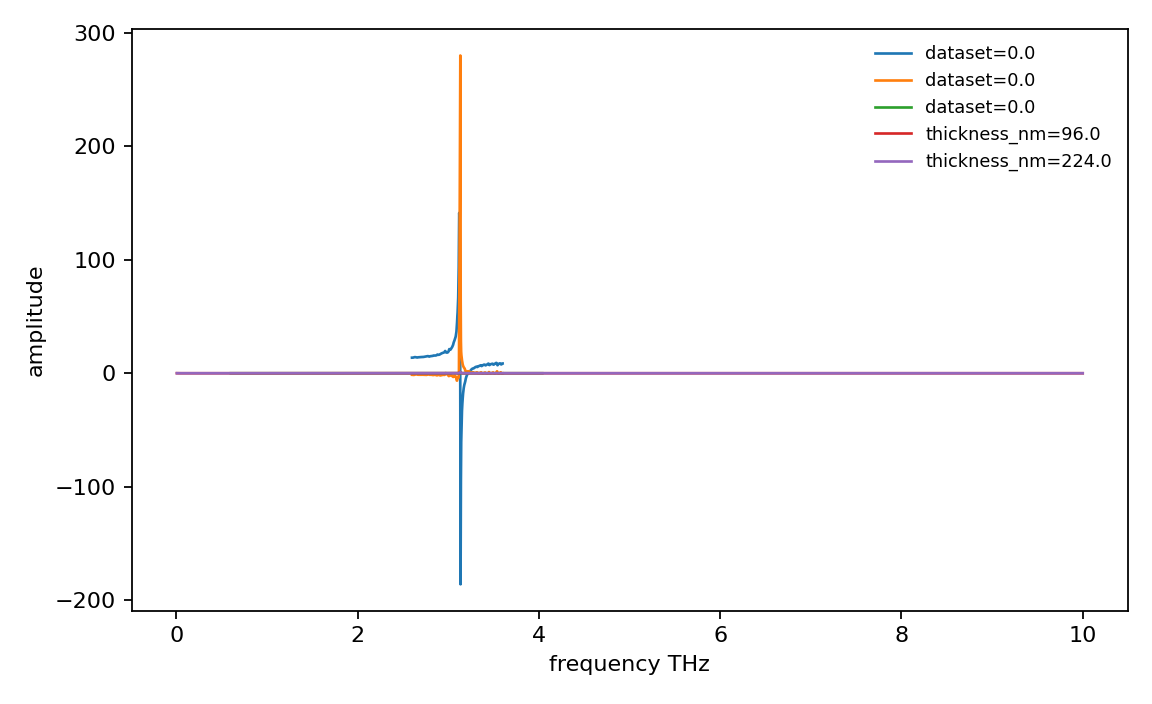
\includegraphics[width=0.88\linewidth]{../experiments/materials_bridge/ferron_coherence_demo/outputs/spectrum_examples.png}
\caption{Example parsed spectra from the public Figshare source-data files.}
\end{figure}

\begin{figure}[ht]
\centering
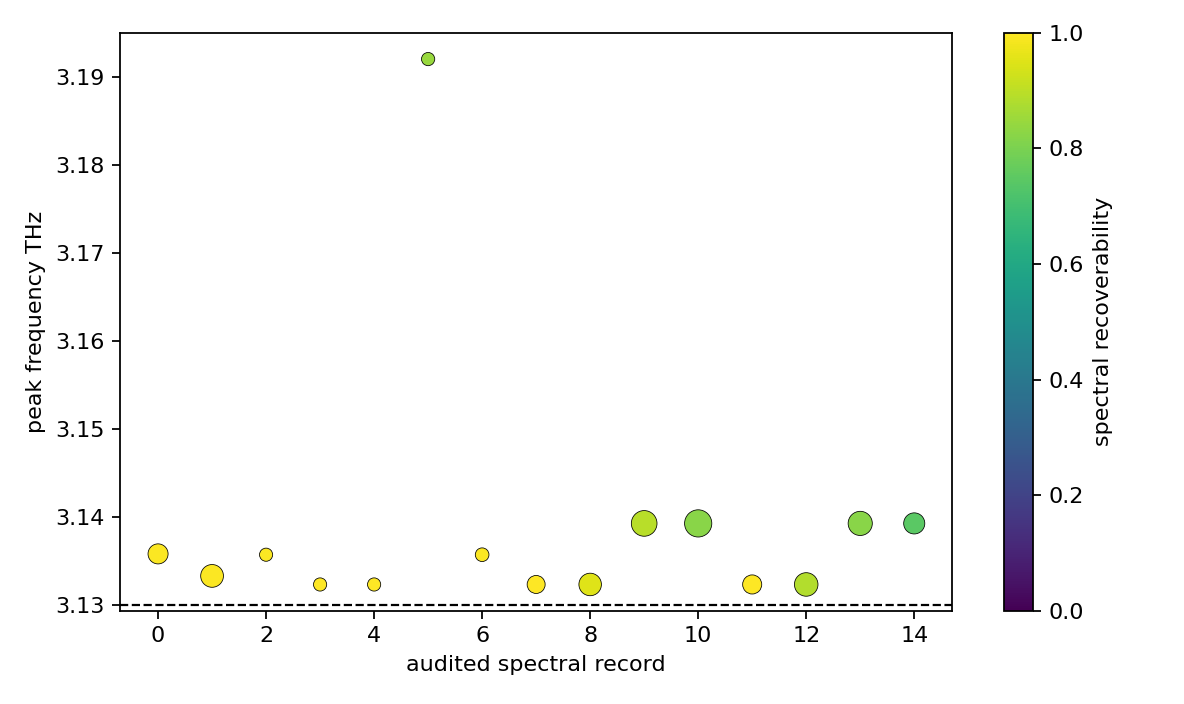
\includegraphics[width=0.88\linewidth]{../experiments/materials_bridge/ferron_coherence_demo/outputs/spectral_peak_map.png}
\caption{Second-pass spectral peak audit. The target-window peak remains near \(3.13\,\mathrm{THz}\) across the audited records.}
\end{figure}

\begin{figure}[ht]
\centering
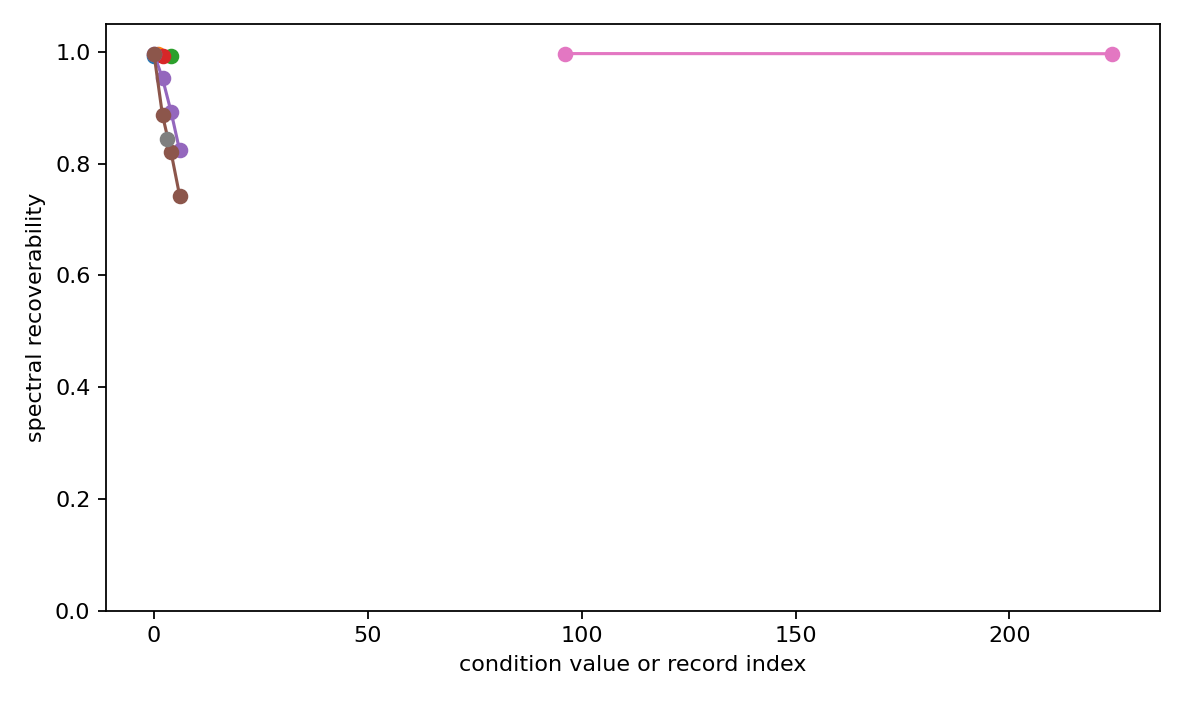
\includegraphics[width=0.88\linewidth]{../experiments/materials_bridge/ferron_coherence_demo/outputs/spectral_recoverability_audit.png}
\caption{Spectral recoverability audit across parsed conditions. No sustained \(k_\star\) collapse is detected under the current proxy thresholds.}
\end{figure}

\begin{figure}[ht]
\centering
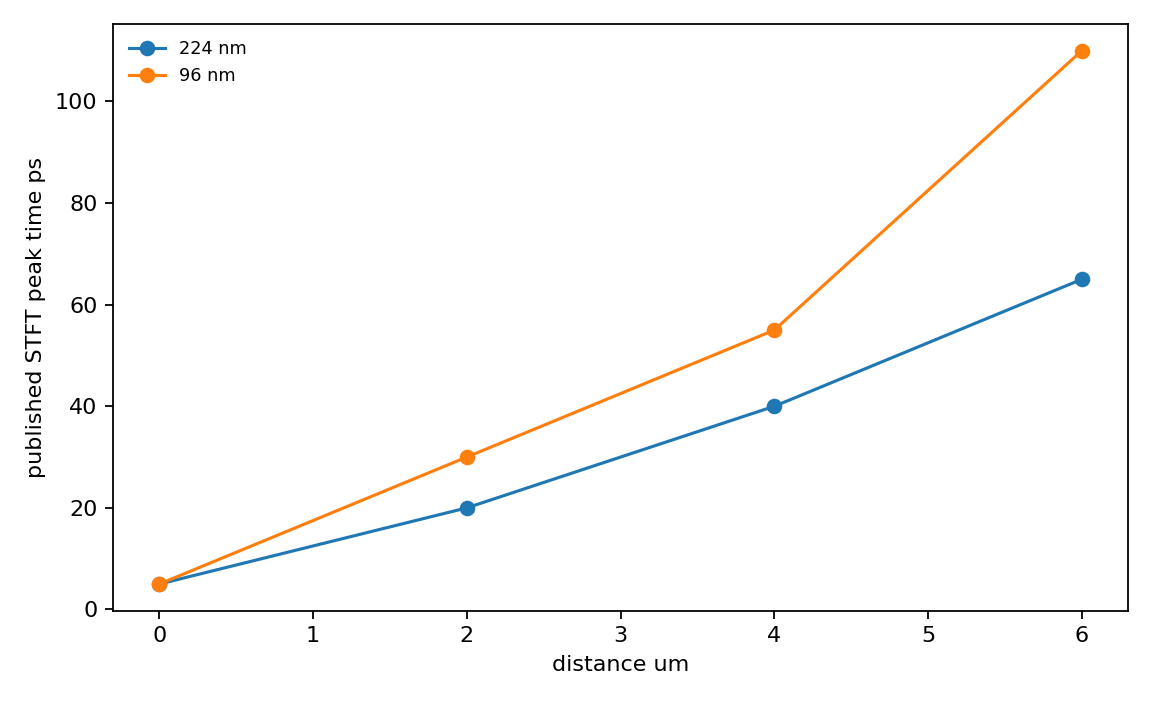
\includegraphics[width=0.88\linewidth]{../experiments/materials_bridge/ferron_coherence_demo/outputs/published_stft_peak_time_vs_distance.png}
\caption{Published Fig. 2d target-band STFT intensity traces: peak time versus distance. These are post-processed target-band traces, not raw time-frequency grids.}
\end{figure}

\begin{figure}[ht]
\centering
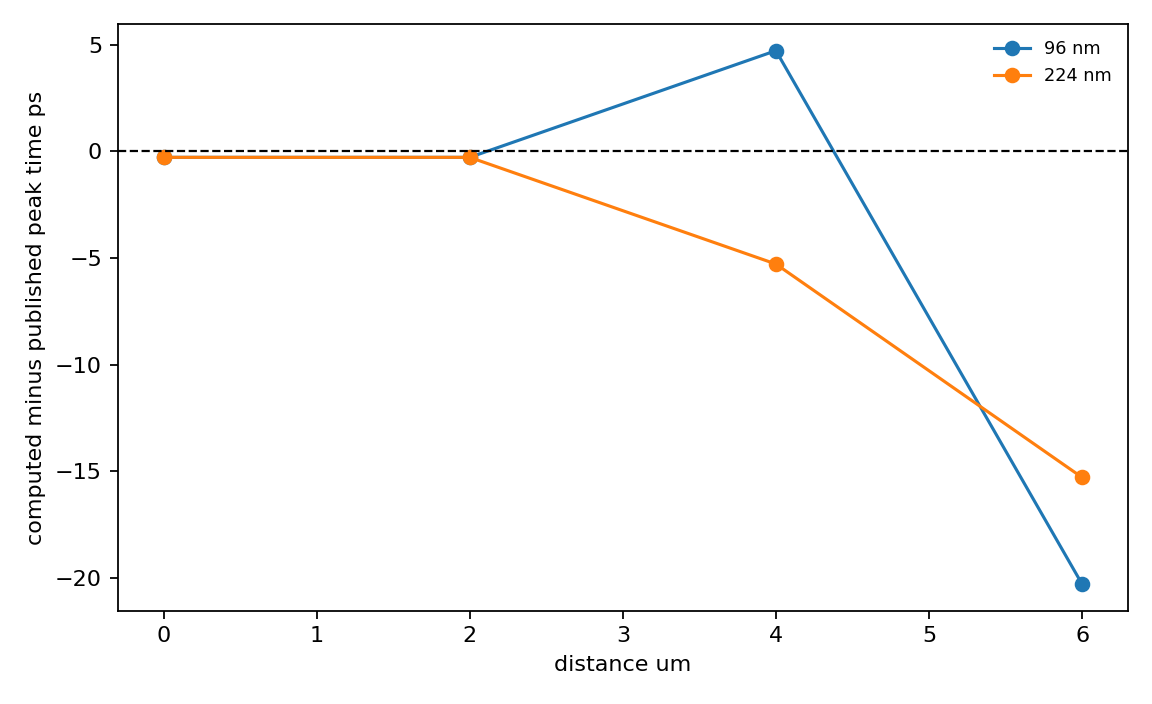
\includegraphics[width=0.88\linewidth]{../experiments/materials_bridge/ferron_coherence_demo/outputs/computed_stft_diagnostic/computed_vs_published_stft_comparison.png}
\caption{Derived computed-from-time-trace STFT target-band envelopes compared with the published Fig. 2d target-band traces.}
\end{figure}

\begin{figure}[ht]
\centering
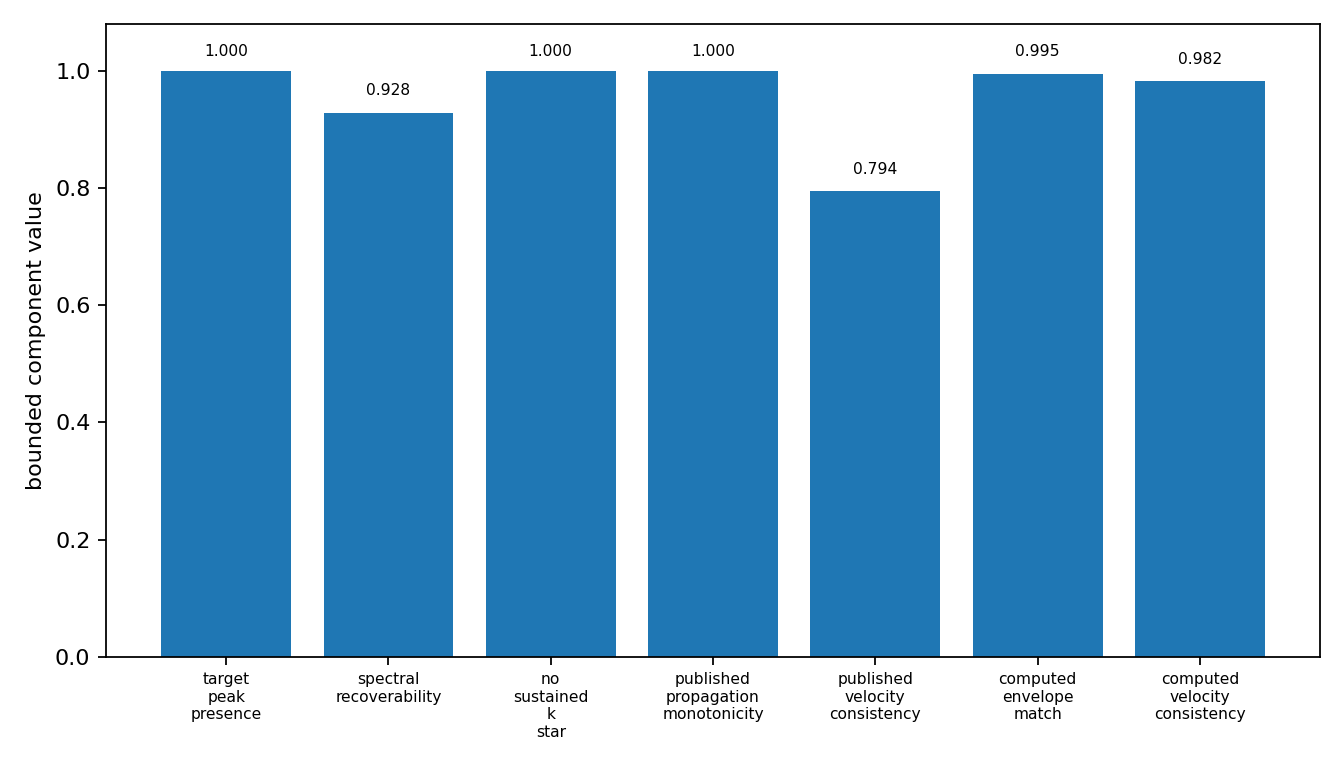
\includegraphics[width=0.88\linewidth]{../experiments/materials_bridge/ferron_coherence_demo/outputs/ferron_harmonic_address_persistence_components.png}
\caption{Unified persistence summary components. The raw STFT grid boundary is recorded separately and is not included as a numeric persistence penalty.}
\end{figure}

\section{Interpretation}

The correct interpretation is narrow:

\begin{quote}
HAOS-IIP Materials Bridge Line A is now running on real ferron / NbOI$_2$ data. The pipeline downloads published Figshare XLSX source data, records provenance, parses time traces and spectra, runs bounded recoverability metrics, and returns \texttt{PASS} as an external-data bridge. The second-pass spectral audit finds the target-window peak in \texttt{15/15} records with mean peak frequency \texttt{3.13893 THz} and mean spectral recoverability \texttt{0.928455}. Under the current proxy thresholds, no \(k_\star\) collapse is detected. The raw STFT audit finds no validated time-frequency grid, so no STFT recoverability claim is made.
\end{quote}

The additional trace and persistence layers refine this without changing the
boundary:

\begin{quote}
The published Fig. 2d target-band traces provide a bounded propagation readout,
and the computed-from-time-trace diagnostic reproduces the target-band envelope
closely enough to serve as a derived reproducibility check. The unified
persistence proxy \texttt{0.957192} is therefore a compact sidecar summary of
peak presence, spectral recoverability, monotonic propagation delay, velocity
consistency, and computed envelope match. It is not a proof of HAOS-IIP, not a
claim that ferrons embody HAOS-IIP, and not a raw STFT-grid claim.
\end{quote}

This matters because the result is not tuned into a dramatic claim. External data comes first. Interpretation comes second.

\section{Artifacts}

\begin{longtable}{p{0.34\linewidth}p{0.52\linewidth}}
\toprule
Artifact & Path \\
\midrule
\endhead
Loader & \path{experiments/materials_bridge/ferron_coherence_demo/ferron_data_loader.py} \\
Metric model & \path{experiments/materials_bridge/ferron_coherence_demo/ferron_recoverability_model.py} \\
Spectral audit & \path{experiments/materials_bridge/ferron_coherence_demo/spectral_feature_audit.py} \\
STFT audit & \path{experiments/materials_bridge/ferron_coherence_demo/stft_feature_audit.py} \\
Computed STFT diagnostic & \path{experiments/materials_bridge/ferron_coherence_demo/ferron_computed_stft_diagnostic.py} \\
Persistence summary & \path{experiments/materials_bridge/ferron_coherence_demo/ferron_harmonic_address_persistence_summary.py} \\
Runner & \path{experiments/materials_bridge/ferron_coherence_demo/run_ferron_coherence_demo.py} \\
Manifest & \path{experiments/materials_bridge/ferron_coherence_demo/data_manifest.json} \\
Validation report & \path{experiments/materials_bridge/ferron_coherence_demo/ferron_coherence_validation.md} \\
Results CSV & \path{experiments/materials_bridge/ferron_coherence_demo/outputs/results.csv} \\
Spectral summary & \path{experiments/materials_bridge/ferron_coherence_demo/outputs/spectral_feature_summary.json} \\
STFT summary & \path{experiments/materials_bridge/ferron_coherence_demo/outputs/stft_feature_summary.json} \\
Published target-band trace summary & \path{experiments/materials_bridge/ferron_coherence_demo/outputs/published_stft_trace_summary.json} \\
Computed STFT summary & \path{experiments/materials_bridge/ferron_coherence_demo/outputs/computed_stft_diagnostic/computed_stft_summary.json} \\
Persistence summary JSON & \path{experiments/materials_bridge/ferron_coherence_demo/outputs/ferron_harmonic_address_persistence_summary.json} \\
Summary JSON & \path{experiments/materials_bridge/ferron_coherence_demo/outputs/summary.json} \\
\bottomrule
\end{longtable}

\section{Conclusion}

Release \texttt{64.1} adds a real external materials-data bridge to HAOS-IIP. It is a bounded operational milestone, not a theory escalation. The ferron / NbOI$_2$ source data loads, parses, hashes, plots, and produces recoverability telemetry. The measured spectral result is stable under the current proxy thresholds: no \(k_\star\), no visible failure, and no early-detection claim. The published target-band STFT intensity traces add a bounded propagation readout, and the computed-from-time-trace diagnostic provides a derived reproducibility check against those traces. The unified persistence proxy is \texttt{0.957192}. The raw STFT audit also says no cleanly: no validated raw STFT/time-frequency grid is present in the downloaded XLSX files, so no raw STFT-grid recoverability claim is made. That non-hyped outcome is the point of the bridge.

\end{document}
